\chapter{Fearful Symmetries} 
\lstset{style=6502Style}

% \newdate{..label..}{..date..}{..info..}
\newcommand\addItem[2]%
{
  \expandafter\def\csname row:#1\endcsname{#2}%
}

% \showItem{..label..}
\newcommand\showItem[1]%
{\expandafter\csname row:#1\endcsname}


% \getItem{..label..}
\newcommand\getItem[1]%
{\noindent
  \text{\showItem{#1}}
  \par
}
% An array of captions 
\addItem{0}{Star One: Y-Axis, X-Y Symmetry, X-Axis Symmetry, Quad Symmetry}
\addItem{1}{The Twist: Y-Axis, X-Y Symmetry, X-Axis Symmetry, Quad Symmetry}
\addItem{2}{La Llamita: Y-Axis, X-Y Symmetry, X-Axis Symmetry, Quad Symmetry}
\addItem{3}{Star Two: Y-Axis, X-Y Symmetry, X-Axis Symmetry, Quad Symmetry}
\addItem{4}{Deltoid: Y-Axis, X-Y Symmetry, X-Axis Symmetry, Quad Symmetry}
\addItem{5}{Diffused: Y-Axis, X-Y Symmetry, X-Axis Symmetry, Quad Symmetry}
\addItem{6}{Multi-Cross: Y-Axis, X-Y Symmetry, X-Axis Symmetry, Quad Symmetry}
\addItem{7}{Pulsar: Y-Axis, X-Y Symmetry, X-Axis Symmetry, Quad Symmetry}
\addItem{8}{Custom Pattern 1: Y-Axis, X-Y Symmetry, X-Axis Symmetry, Quad Symmetry}
\addItem{9}{Custom Pattern 2: Y-Axis, X-Y Symmetry, X-Axis Symmetry, Quad Symmetry}
\addItem{10}{Custom Pattern 3: Y-Axis, X-Y Symmetry, X-Axis Symmetry, Quad Symmetry}
\addItem{11}{Custom Pattern 4: Y-Axis, X-Y Symmetry, X-Axis Symmetry, Quad Symmetry}
\addItem{12}{Custom Pattern 5: Y-Axis, X-Y Symmetry, X-Axis Symmetry, Quad Symmetry}
\addItem{13}{Custom Pattern 6: Y-Axis, X-Y Symmetry, X-Axis Symmetry, Quad Symmetry}
\addItem{14}{Custom Pattern 7: Y-Axis, X-Y Symmetry, X-Axis Symmetry, Quad Symmetry}

There are 4 possible symmetries for displaying patterns in Psychedelia. As we saw when
reviewing the code for the magazine listing the painting of the symmetries is managed
by \icode{PaintPixelForCurrentSymmetry}. There it was hardcoded to use a simple
reflection symmetry along the X-axis, but the commercial version of Psychedelia has to
go a little further and support along all three possible axes. 

Now that the player can change the active symmetry at any time, there is a little more
book-keeping for Psychedelia to do in terms of recognizing the active symmetry for each
step in the pattern's evolution. In this chapter we'll take a look at how this 
\textit{fascinating} bit of accounting works and console ourselves the while with some
pretty pictures of the symmetry rendering in operation. First, a couple of pretty pictures.
Then some potentially tedious unpacking of code.

\foreach \l in {0,...,1}
{
  \begin{figure}[H]
      \centering
        \vspace*{-6cm}
        \hspace*{-8cm}
        \includegraphics[width=20cm]{src/symmetries/pattern\l_1-45.png}%
        \hspace*{-12cm}
        \includegraphics[width=20cm]{src/symmetries/pattern\l_2-45.png}\\
        \vspace*{-13cm}
        \hspace*{-7cm}
        \includegraphics[width=20cm]{src/symmetries/pattern\l_3-45.png} \\
        \vspace*{-20cm}
        \includegraphics[width=20cm]{src/symmetries/pattern\l_4-45.png}
        \vspace*{-4cm}
  \caption*{\getItem{\l}}
  \end{figure}

}%

\clearpage
\begin{lstlisting}
;-------------------------------------------------------
; CheckKeyboardInput
;-------------------------------------------------------
CheckKeyboardInput   
        ...
        LDA lastKeyPressed
        ...
MaybeSPressed   
        CMP #KEY_S ; 'S' pressed.
        BNE MaybeLPressed

        ; Check if shift was pressed too.
        LDA shiftPressed
        AND #$01
        BEQ JustSPressed

        LDA tapeSavingInProgress
        BNE JustSPressed
        ; Shift + S pressed: Save.
        JMP PromptToSave
        ; Returns

        ; 'S' pressed. 
JustSPressed   
        INC currentSymmetrySetting
        LDA currentSymmetrySetting
        CMP #$05
        BNE SetUpYRegisterToGetText
        LDA #$00
        STA currentSymmetrySetting

SetUpYRegisterToGetText   
        ASL 
        ASL 
        ASL 
        ASL 
        TAY 
        JSR ClearLastLineOfScreen

        ; currentSymmetrySetting is in Y
        LDX #$00
WriteSymmetryDescription   
        LDA txtSymmetrySettingDescriptions,Y
        STA lastLineBufferPtr,X
        INY 
        INX 
        CPX #$10
        BNE WriteSymmetryDescription

        JMP WriteLastLineBufferToScreen
        ;Returns
\end{lstlisting}
\clearpage

\textbf{Lines 1189-1231. \icode{\textbf{MaybeSPressed}}:} This is the routine that detects when the player has selected a new
symmetry by pressing the 'S' key. It is part of the much larger routine \icode{CheckKeyboardInput} which periodically checks
for keyboard input by polling the byte at address \icode{\$00C5} (which we label \icode{lastKeyPressed}). This address always
contains the value of the most recently pressed key on the keyboard.

If Shift was pressed the user is actually looking to trigger a save, in which case execution passes to \icode{PromptToSave}.

Otherwise we increment \icode{currentSymmetrySetting}, which is the variable we use for storing the currently selected symmetry.
Each press of the 'S' key increments the value of \icode{currentSymmetrySetting} until it reaches 5. Once that happens, we 
reset it to zero again (\icode{LDA \#\$00; STA currentSymmetrySetting}).

\textbf{Lines 1214-1219. \icode{\textbf{SetUpYRegisterToGetText}}:} What is the series of \icode{ASL} instructions doing? A tricky
piece of business of course. We have loaded \icode{currentSymmetrySetting} to the \icode{A} register (\icode{LDA currentSymmetrySetting}) and it has a value between 0 and 4.
\icode{ASL} performs a leftward bit-shift on the \icode{A} register. A single left-shift has an interesting property - it doubles the
value of the byte. A second left-shift will double it again, and so on. So our four {ASL} instructions have the effect of turning 1 into
16, 2 into 32, 3 into 48, and 4 into 64. This has the very useful effect of giving us an index into the description of each symmetry!

\begin{lstlisting}
txtSymmetrySettingDescriptions 
        .TEXT 'NO SYMMETRY     ' ; Starts at index 0
        .TEXT 'Y-AXIS SYMMETRY ' ; Starts at index 16
        .TEXT 'X-Y SYMMETRY    ' ; Starts at index 32
        .TEXT 'X-AXIS SYMMETRY ' ; Starts at index 48
        .TEXT 'QUAD SYMMETRY   ' ; Starts at index 64
\end{lstlisting}

So when we take our resulting value and load it into the \icode{Y} register all our \icode{WriteSymmetryDescription} needs to do is start at the 
index given by \icode{Y} and write out the next 16 bytes to the screen, displaying the selected symmetry briefly to the player.


\clearpage
\foreach \l in {2,...,3}
{
  \begin{figure}[H]
      \centering
        \vspace*{-6cm}
        \hspace*{-8cm}
        \includegraphics[width=20cm]{src/symmetries/pattern\l_1-45.png}%
        \hspace*{-12cm}
        \includegraphics[width=20cm]{src/symmetries/pattern\l_2-45.png}\\
        \vspace*{-13cm}
        \hspace*{-7cm}
        \includegraphics[width=20cm]{src/symmetries/pattern\l_3-45.png} \\
        \vspace*{-20cm}
        \includegraphics[width=20cm]{src/symmetries/pattern\l_4-45.png}
        \vspace*{-4cm}
  \caption*{\getItem{\l}}
  \end{figure}

}%

\clearpage
\begin{lstlisting}
;-------------------------------------------------------
; PaintPixelForCurrentSymmetry
;-------------------------------------------------------
PaintPixelForCurrentSymmetry   
        ; First paint the normal pattern without any
        ; symmetry.
        LDA pixelXPosition
        PHA 
        LDA pixelYPosition
        PHA 
        JSR PaintPixel

        LDA currentSymmetrySettingForStep
        BNE HasSymmetry

CleanUpAndReturnFromSymmetry   
        PLA 
        STA pixelYPosition
        PLA 
        STA pixelXPosition
        RTS 

        RTS

HasSymmetry   
        CMP #X_AXIS_SYMMETRY
        BEQ XAxisSymmetry

        ; Has a pattern to paint on the Y axis
        ; symmetry so prepare for that.
        LDA #$27
        SEC 
        SBC pixelXPosition
        STA pixelXPosition

        ; If it has X_Y_SYMMETRY then we just 
        ; need to paint that, and we're done.
        LDY currentSymmetrySettingForStep
        CPY #X_Y_SYMMETRY
        BEQ XYSymmetry

        ; If we're here it's either Y_AXIS_SYMMETRY
        ; or QUAD_SYMMETRY so we can paint a pattern
        ; on the Y axis.
        JSR PaintPixel

\end{lstlisting}
\clearpage

\textbf{Lines 348-548. \icode{\textbf{PaintPixelForCurrentSymmetry}}:} This routine seems a lot more convoluted than it
ought to be. What it needs to do is figure out which of the four symmetries it ought to paint and paint them.

\textbf{Lines 352,354. \icode{\textbf{PHA}}:} Notice that we're pushing the values in \icode{pixelXPosition} and \icode{pixelYPosition}
on to the stack. The reason for this is that we may have to modify one or both of \icode{pixelXPosition/pixelYPosition} when
painting the symmetries so we can later pull them back off the stack (\icode{PLA}) and restore each to their original
values when we're finished.

\textbf{Lines 348-548. \icode{\textbf{CleanUpAndReturnFromSymmetry}}:} The simplest case is easiest. If we get to here
the symmetry setting just requires one pattern to be drawn (\icode{NO SYMMETRY}) so after calling \icode{PaintPixel}
we can return early.

\textbf{Lines 369-548. \icode{\textbf{HasSymmetry}}:} We know what this section ought to be doing, but you really do have
to stare at it quite a long time to work out how it's doing it. What it ought to be doing is painting a pixel reflected on one or more
of the X and Y axes depending on the setting of \icode{currentSymmetrySettingForStep}. In the process it jumps around a bit,
shuffles values on and off the stack and has a couple of points where the routine can return early. None of this really aids
the cause of understanding.

\clearpage
\begin{lstlisting}
        ; If it's Y_AXIS_SYMMETRY we're done and can 
        ; return.
        LDA currentSymmetrySettingForStep
        CMP #Y_AXIS_SYMMETRY
        BEQ CleanUpAndReturnFromSymmetry

        ; Has QUAD_SYMMETRY so the remaining steps are
        ; to paint two more: one on our X axis and one
        ; on our Y axis.

        ; First we do the Y axis.
        LDA #NUM_ROWS
        SEC 
        SBC pixelYPosition
        STA pixelYPosition
        JSR PaintPixel

        ; Paint one on the X axis.
PaintXAxisPixelForSymmetry    
        PLA 
        TAY 
        PLA 
        STA pixelXPosition
        TYA 
        PHA 
        JSR PaintPixel
        PLA 
        STA pixelYPosition
        RTS 

XAxisSymmetry   
        LDA #NUM_ROWS
        SEC 
        SBC pixelYPosition
        STA pixelYPosition
        JMP PaintXAxisPixelForSymmetry

XYSymmetry   
        LDA #NUM_ROWS
        SEC 
        SBC pixelYPosition
        STA pixelYPosition
        JSR PaintPixel
        PLA 
        STA pixelYPosition
        PLA 
        STA pixelXPosition
        RTS 
\end{lstlisting}
\clearpage

\textbf{Lines 369-548. \icode{\textbf{XAxisSymmetry}}:} It's called \icode{X-AXIS SYMMETRY} but the reflection is on the Y Axis, i.e.
on the vertical. Maybe it's called that because the patterns share the same X-coordinate? Either way, it's a confusing name for what
it is.

\begin{figure}[H]
    \centering
      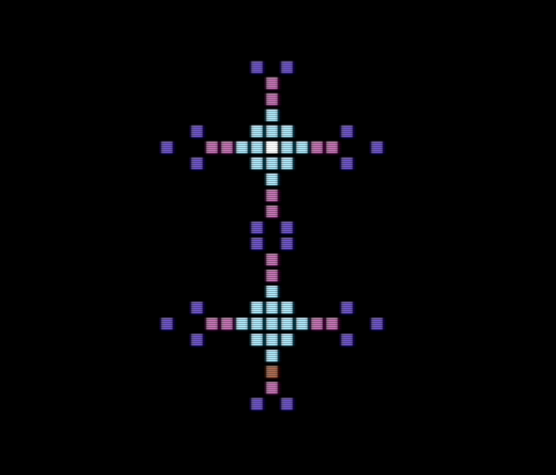
\includegraphics[height=5cm]{src/symmetries/xaxis.png}
  \caption*{\icode{X-AXIS SYMMETRY} - despite the name it's along the Y axis.}
\end{figure}

So what we actually want to do here is reflect the pattern on the Y axis. This means manipulating \icode{pixelYPosition} so that it's
offset halfway down the screen. 

\textbf{Lines 369-548. \icode{\textbf{PaintXAxisPixelForSymmetry}}:} 

\clearpage
\foreach \l in {4,...,14}
{
  \begin{figure}[H]
      \centering
        \vspace*{-6cm}
        \hspace*{-8cm}
        \includegraphics[width=20cm]{src/symmetries/pattern\l_1-45.png}%
        \hspace*{-12cm}
        \includegraphics[width=20cm]{src/symmetries/pattern\l_2-45.png}\\
        \vspace*{-13cm}
        \hspace*{-7cm}
        \includegraphics[width=20cm]{src/symmetries/pattern\l_3-45.png} \\
        \vspace*{-20cm}
        \includegraphics[width=20cm]{src/symmetries/pattern\l_4-45.png}
        \vspace*{-4cm}
  \caption*{\getItem{\l}}
  \end{figure}

}%
